%====================================================================
\subsection{Regular PLN}
%====================================================================
\frame{\frametitle{Regular PLN} \pause

  \paragraph{Fruit flies in La R\'eunion.} \refer{FHC21}
  $p = 8$ fly species: 
  \begin{itemize}
    \setlength{\itemsep}{0.5\baselineskip}
    \item 4 generalists ({\it B. zonata}, {\it C. capitata}, {\it C. catoirii} and {\it C. quilicii}),  
    \item 3 specialists of Cucurbitaceae ({\it D. ciliatus}, {\it D. demmerezi} and {\it Z. cucurbitae}), 
    \item 1 specialist of Solanaceae ({\it N. cyanescens}).
  \end{itemize}
  
  \bigskip
  $n \simeq 5000$ plants
  
  \pause \bigskip \bigskip
  \paragraph{Questions.}
  \begin{itemize}
    \setlength{\itemsep}{0.5\baselineskip}
    \item Do sympatric species do actually share the same niche (e.g. plants)?
    \item Do climatic factors affect their respective abundances?
    \item Are species actually in competition?
  \end{itemize}
}

%====================================================================
\frame{\frametitle{Fruit flies in La R\'eunion} 

  \paragraph{Regular PLN model.} Estimated covariance matrices $\Sigma$:
  $$
  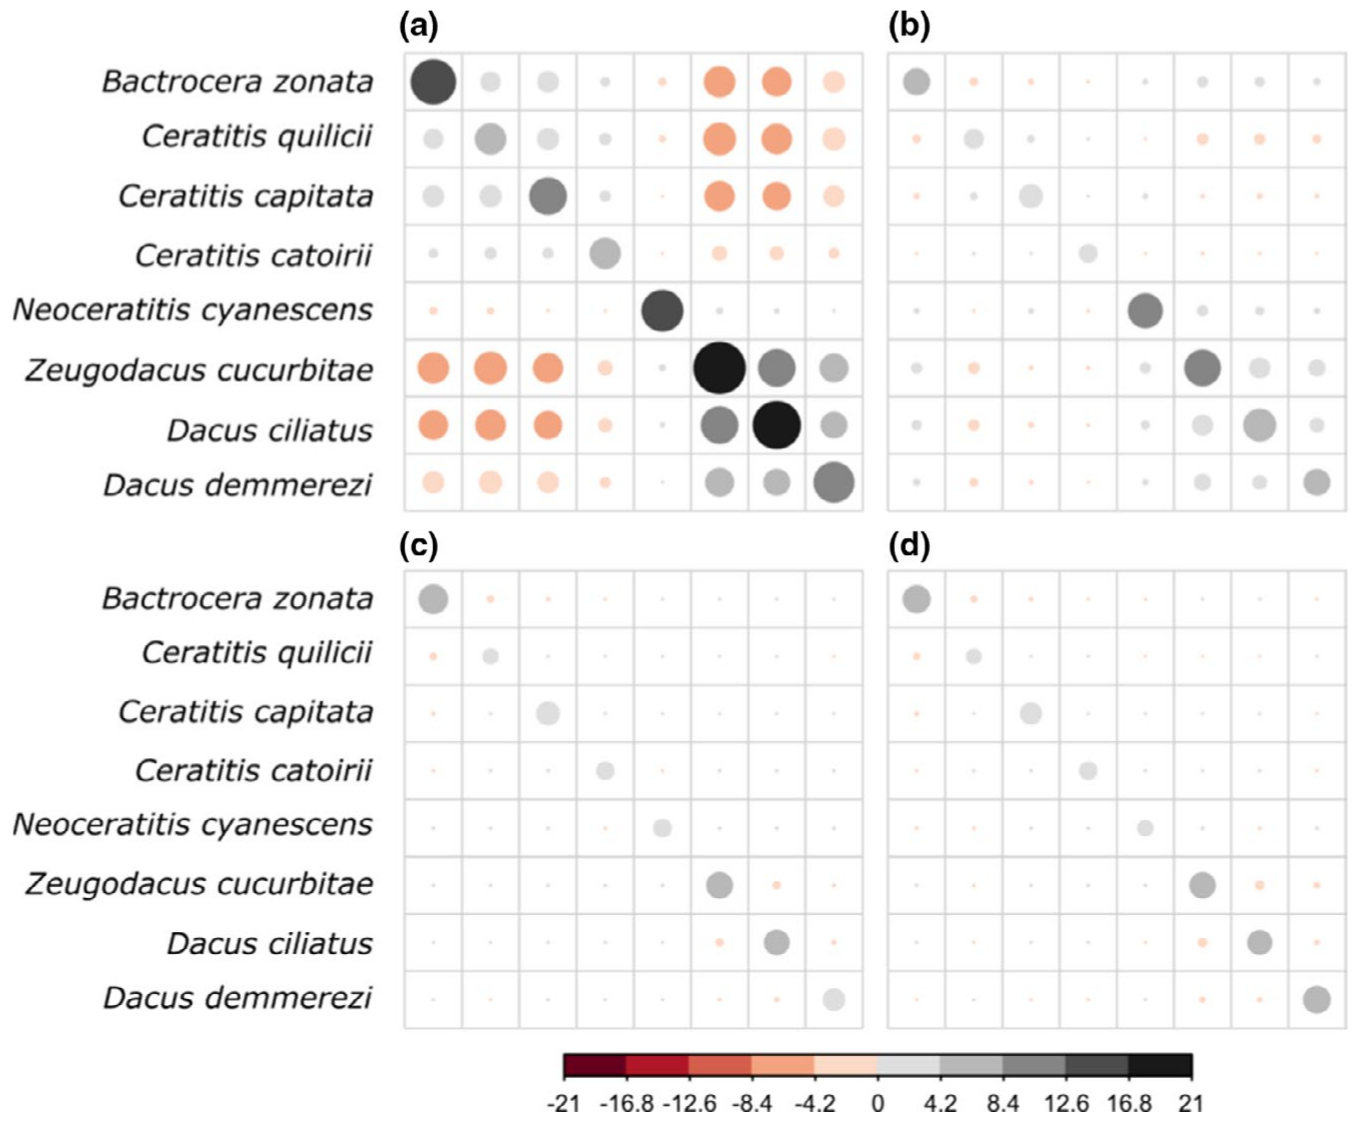
\includegraphics[width=.5\textwidth]{\figeco/FHC20-EcolLetters-Fig2}
  $$
  $$
  \begin{tabular}{clcl}
    \qquad & (a) No covariate & \qquad \qquad & (b) Climat \\
    \qquad & (c) Plant species & & (d) Plant species and climat
  \end{tabular}
  $$
  
  \bigskip
  \ra Weak competition among species specialists of the same plant.
}

